\chapter{模板配置与软件环境配置}

\section{模板配置}
根据毕业类型选择不同的模板,\verb+\documentclass[master]{hdu-thesis}[]+中不同的模式配置对应不同的模板,具体见下图或README.md。
 \begin{figure}[!htb]
  \centering
  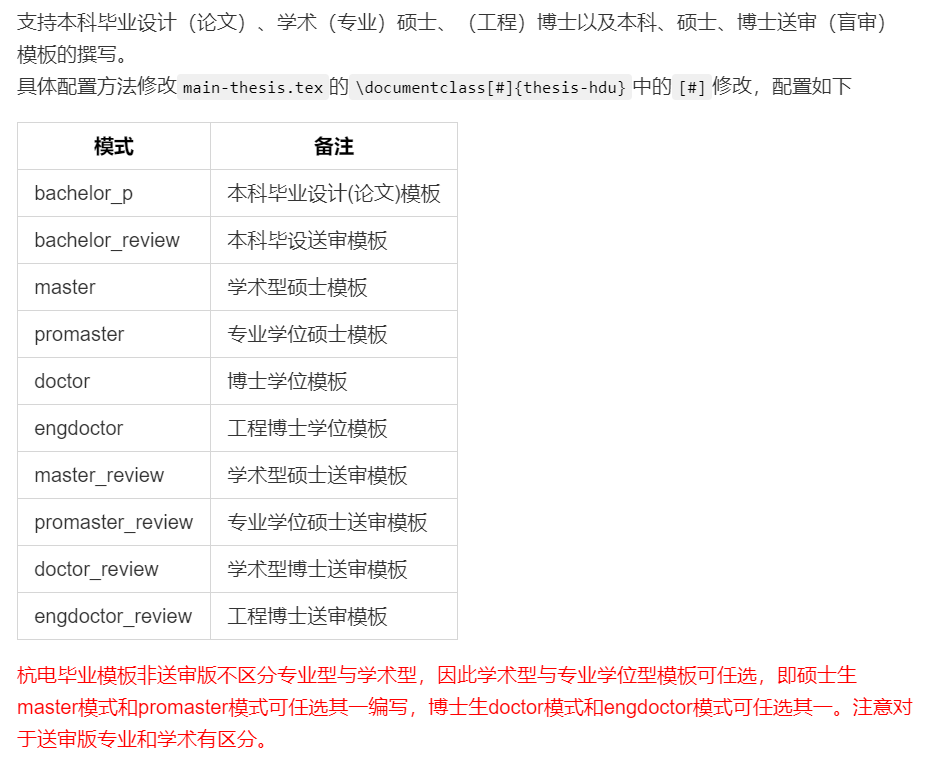
\includegraphics[width=1\textwidth]{模板选择}
  \caption{documentclass模板配置}
\end{figure}

\section{软件配置}
\textcolor{red}{下载最新texlive配合vscode}
其中,texlive配合vscode可参考以下网址:\\
\url{https://zhuanlan.zhihu.com/p/166523064},或者 \href{https://zhuanlan.zhihu.com/p/38178015}{知乎-使用VSCode编写LaTeX}。

\textcolor{red}{VSCode的latex插件安装后的具体配置,参考README.md文档末尾说明。}

pdf预览可用\\
vscode的latex-workshop.view.pdf.viewer预览,支持双击反向搜索。

配置完如下图所示,红色是需要用到的指令(如图\ref{fig_vs_latex}),
 \begin{figure}[!htb]
  \centering
  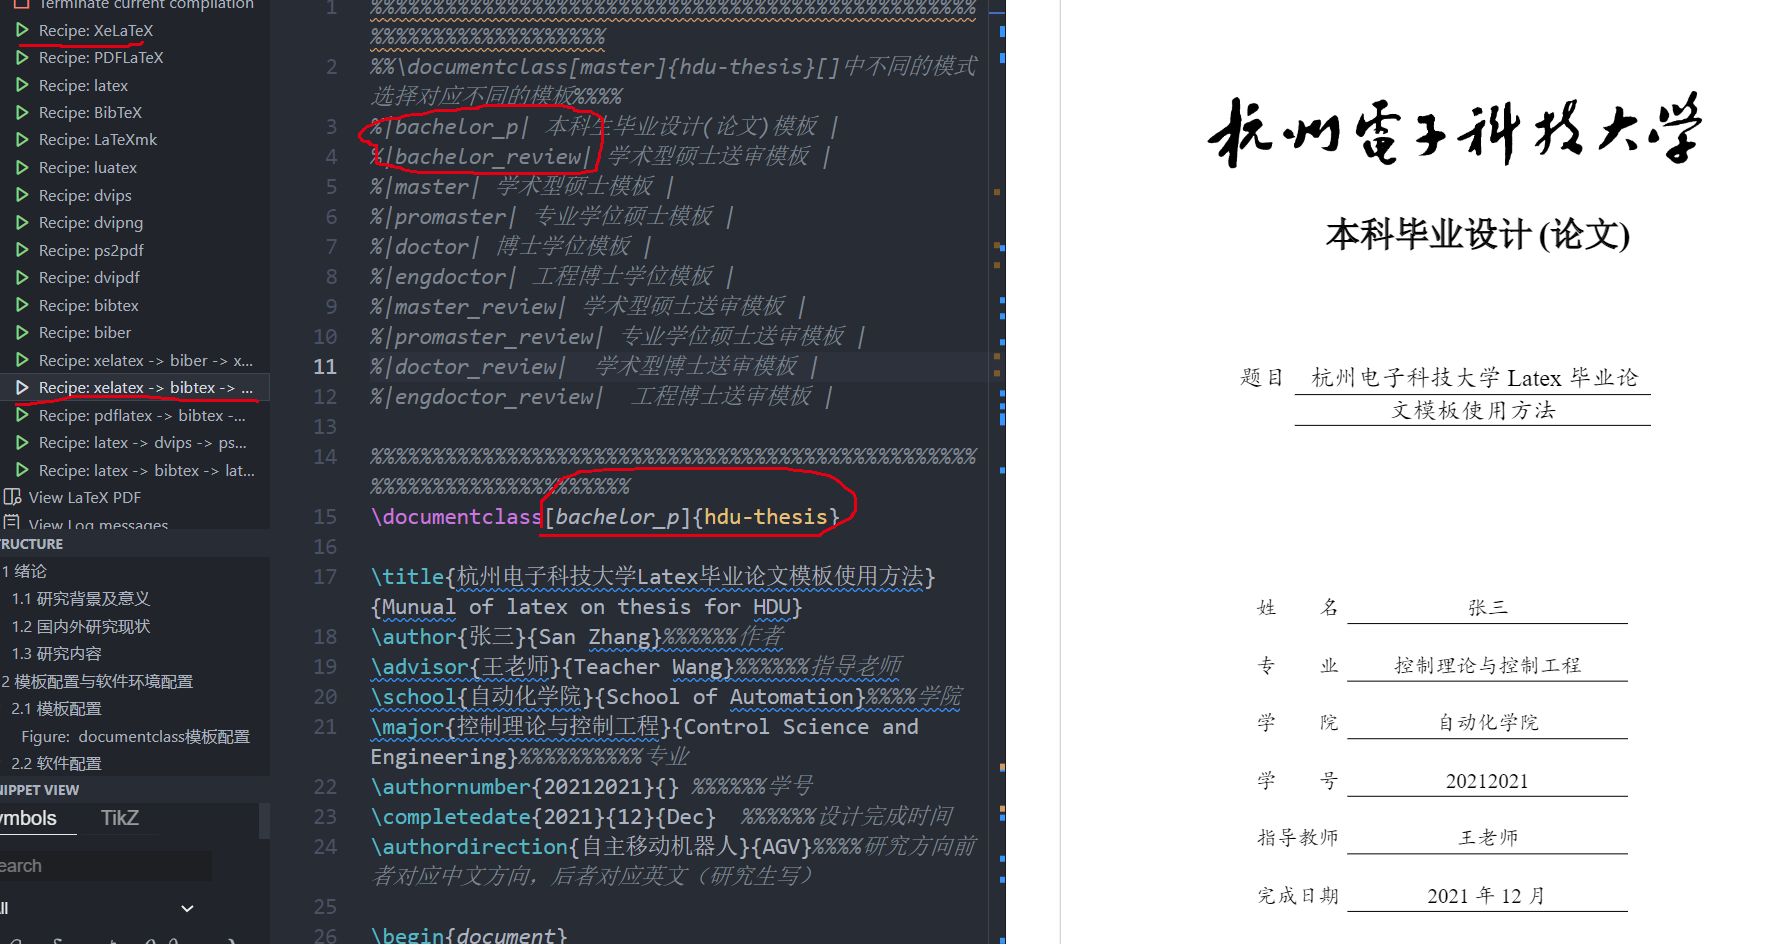
\includegraphics[width=1\textwidth]{vscode-latex}
  \caption{vscode配置latex}
  \label{fig_vs_latex}
\end{figure}

\subsection{指令}
\subsubsection{编译指令}
如果先不编译参考文献,只编译正文的话只需点Xelatex,想编译参考文献并生成参考文献目录,需依次点击 Xelatex-B-Xelatex-Xelatex\footnote{脚注}。指令见图\ref{fig_vs_latex}。

